% ****** Start of file apssamp.tex ******
%
%   This file is part of the APS files in the REVTeX 4.1 distribution.
%   Version 4.1r of REVTeX, August 2010
%
%   Copyright (c) 2009, 2010 The American Physical Society.
%
%   See the REVTeX 4 README file for restrictions and more information.
%
% TeX'ing this file requires that you have AMS-LaTeX 2.0 installed
% as well as the rest of the prerequisites for REVTeX 4.1
%
% See the REVTeX 4 README file
% It also requires running BibTeX. The commands are as follows:
%
%  1)  latex apssamp.tex
%  2)  bibtex apssamp
%  3)  latex apssamp.tex
%  4)  latex apssamp.tex
%
\documentclass[%
 reprint,
superscriptaddress,
%groupedaddress,
%unsortedaddress,
%runinaddress,
%frontmatterverbose, 
%preprint,
%showpacs,preprintnumbers,
%nofootinbib,
%nobibnotes,
%bibnotes,
 amsmath,amssymb,
 prl,
% aps,
%pra,
%prb,
%rmp,
%prstab,
%prstper,
%floatfix,
]{revtex4-1}

\usepackage{graphicx}% Include figure files
\usepackage{dcolumn}% Align table columns on decimal point
\usepackage{bm}% bold math
\usepackage{color}
\usepackage{pgfplots} 
\usepackage{tikzscale}
\pgfplotsset{compat=newest} 
%\usepackage{hyperref}% add hypertext capabilities
%\usepackage[mathlines]{lineno}% Enable numbering of text and display math
%\linenumbers\relax % Commence numbering lines

%\usepackage[showframe,%Uncomment any one of the following lines to test 
%%scale=0.7, marginratio={1:1, 2:3}, ignoreall,% default settings
%%text={7in,10in},centering,
%%margin=1.5in,
%%total={6.5in,8.75in}, top=1.2in, left=0.9in, includefoot,
%%height=10in,a5paper,hmargin={3cm,0.8in},
%]{geometry}

\begin{document}
\tikzset{font=\fontsize{15}{22.4}\selectfont}
%\preprint{APS/123-QED}

\title{Stabilisation of the Arrival Time of a High Energy Electron Beam at the 
50~fs Level}
%\thanks{A footnote to the article title}%

\author{J.~Roberts}
\email{Corresponding author Jack.Roberts@cern.ch}
\affiliation{John Adams Institute,University of Oxford}
\affiliation{CERN, Geneva}
%\altaffiliation{CERN, Geneva.}

\author{P.~Burrows}
\affiliation{John Adams Institute,University of Oxford}

\author{G.~Christian}
\affiliation{John Adams Institute,University of Oxford}

\author{R.~Corsini}
\affiliation{CERN, Geneva}

\author{A.~Ghigo}
\affiliation{INFN/LNF, Frascati}

\author{F.~Marcellini}
\affiliation{INFN/LNF, Frascati}

\author{C.~Perry}
\affiliation{John Adams Institute,University of Oxford}

\author{P.~Skowronski}
\affiliation{CERN, Geneva}

\date{\today}

\begin{abstract}
CLIC, a proposed future linear electron-positron collider, and other machines 
such as XFELs, place tight tolerances on the phase stabilities of their beams. 
CLIC proposes the use of a novel, high bandwidth and low latency, `phase 
feedforward' system required to achieve a phase stability of 
\(0.2^\circ\)~at~12~GHz, or 
about 50~fs. This work documents the results from operation of a prototype 
phase 
feedforward system at the CLIC test facility CTF3, with 30~MHz bandwidth and a 
total hardware latency of 100~ns. New phase monitors with 
30~fs resolution, 20~kW amplifiers with 47~MHz bandwidth, and electromagnetic 
kickers have been designed and installed for the system. The system utilises a 
chicane in the beamline, for which new optics have been created and 
commissioned. The prototype has demonstrated CLIC-level phase stability, 
reducing an initial rms phase variation of \(0.92\pm0.04^\circ\) to 
\(0.20\pm0.01^\circ\) across a duration of 10~minutes.
\end{abstract}

%\pacs{Valid PACS appear here}% PACS, the Physics and Astronomy
%                             % Classification Scheme.
%\keywords{Suggested keywords}%Use showkeys class option if keyword
                              %display desired
\maketitle

%\tableofcontents

\section{\label{s:intro}Introduction}

CLIC \cite{CLICCDR} is a proposal for a future linear electron positron 
collider that uses a 
novel two 
beam acceleration concept to achieve a high accelerating gradient of 100~MV/m 
and a collision energy of up to 3 TeV. In this concept the 12~GHz RF power used 
to accelerate the high energy colliding beams is extracted from high intensity 
drive beams.

CLIC's luminosity quickly drops if the RF phase jitters with respect to the 
main beam, causing energy errors and subsequent beam size growth at the 
interaction point. The RF phase 
stability must be \(0.2^\circ\)~at~12~GHz (around 50~fs) or better to limit the 
luminosity loss 
to below 1\% \cite{CLICCDR}.  However, the phase stability of the drive beams 
cannot be 
guaranteed to be better than \(2^\circ\)~at~12~GHz. CLIC therefore requires a 
``phase feedforward'' (PFF) 
system that will reduce the drive beam phase jitter (rms) by an order of 
magnitude. Other machines, such as XFELs, have similar phase stability 
requirements.

The PFF system poses many challenges, particularly in terms of the hardware 
bandwidth (\textgreater17.5~MHz \cite{Gerber2015}), power (500~kW amplifiers) 
and latency 
requirements. A prototype 
PFF 
system 
has therefore 
been designed, commissioned and operated at the CLIC 
test facility CTF3, at CERN, to prove its feasibility. The prototype system 
follows the same concept as the proposed CLIC scheme, and is the focus of this 
work. 

CTF3 provides a 135~MeV electron beam bunched at 3~GHz with a pulse length of 
1.2~\(\mathrm{\mu s}\) and a pulse repetition rate of 0.8~Hz. Further details 
on the CTF3 facility can be found in [REF]. All phases quoted 
in the paper are given in degrees at 12~GHz.

\section{\label{s:ctfLayout}System Design}

\begin{figure*}
	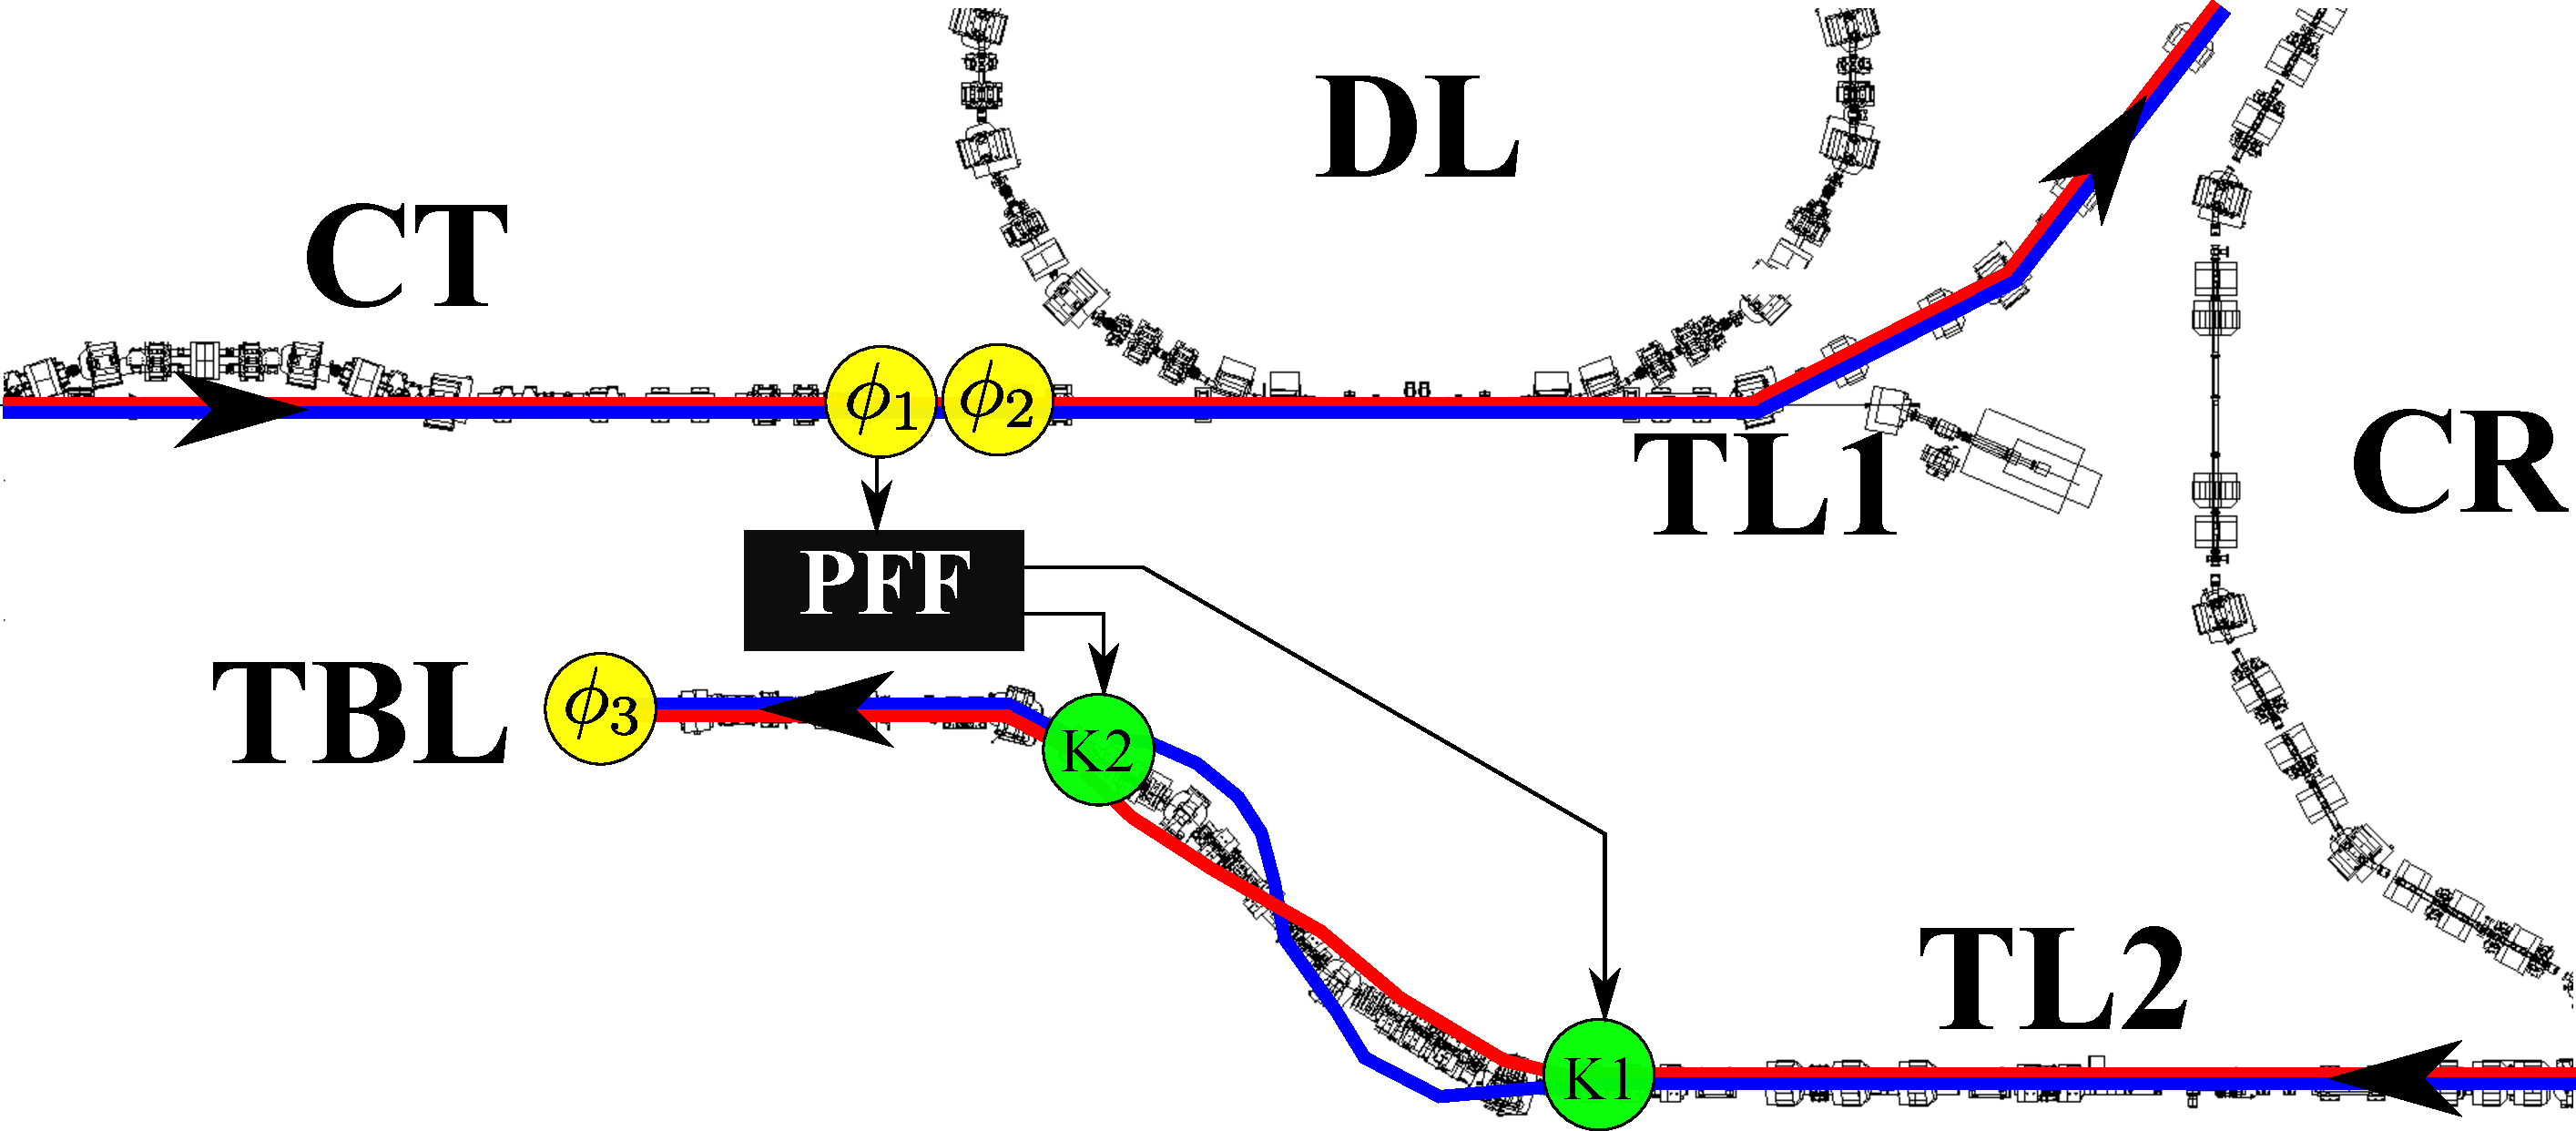
\includegraphics[width=\textwidth]{figs/ctfpffLayout}% Here is how to 
	%import EPS art
	\caption{\label{fig:pffLayout}Schematic of the PFF prototype at CTF3, 
	showing the approximate location of the phase monitors (\(\phi_1\) , 
	\(\phi_2\) and \(\phi_3\)) and
		the kickers (K1 and K2). The black box “PFF” represents the calculation 
		and output of the correction, including the phase monitor
		electronics, feedforward controller and kicker amplifiers. A bunch 
		arriving early at \(\phi_1\) is directed on to a longer path in the TL2 
		chicane
		using the kickers (blue trajectory), whereas a bunch arriving late will 
		be directed on to a shorter path (red trajectory). }
\end{figure*}

A schematic of the PFF system is shown in Fig.~\ref{fig:pffLayout}. The system 
corrects the phase using two electromagnetic kickers installed 
before the first and last dipole in a four bend chicane (in the TL2 transfer 
line). The beam's path length 
through the chicane depends on the magnitude and polarity of the voltage 
applied to the kickers. The phase is measured using a monitor upstream of 
the chicane (in the CT beam line), and then corrected by setting the kicker 
voltage to deflect bunches arriving early at the phase monitor on to longer 
trajectories in the chicane, and bunches arriving late on to shorter 
trajectories. Downstream of the chicane, in the TBL line, another phase monitor 
is placed to measure the effects of the correction.

The beam time of flight between the upstream phase monitor and the first kicker 
in the chicane is 380~ns. By bypassing the combiner ring (CR) and TL1 transfer 
line (see Fig.~\ref{fig:pffLayout}) the total cable length required to 
transport signals between the monitor and kickers is shorter, approximately 
250~ns. The PFF correction in the chicane can therefore be applied to the same 
bunch initially measured at the phase monitor, providing the total system 
hardware latency is less than 130~ns. 

\subsection{\label{ss:hardware}Hardware}

The PFF system uses three phase monitors, two electromagnetic kickers, kicker 
amplifiers and a digitiser/feedforward controller.

The three phase monitors \cite{phMonEuCard} are designed and built by INFN 
Frascati, with the 
associated electronics built by CERN. The monitors are 12~GHz resonating 
cavities with a dipole and monopole mode present. The output from opposing 
vertical pairs of feedthroughs are summed in hybrids to create a position 
independent signal. This signal is split and mixed with a reference 12~GHz 
signal in eight separate mixers. The output from the eight mixers is combined, 
allowing a resolution of \(0.12^\circ\) to be 
achieved whilst maintaining linearity between \(\pm70^\circ\). The quoted 
resolution 
is determined by 
comparing the measurements of the two adjacent upstream monitors (installed in 
the CT 
line, see Fig.~\ref{fig:pffLayout}).

The two electromagnetic stripline kickers \cite{kickerIPAC11} were also 
designed and built by INFN 
Frascati,  
and are based on the DAFNE design. Each kicker is approximately 1~m in length, 
with a horizontal strip separation of 40~mm. A voltage of 1.26~kV applied to 
the 
downstream end of the kicker strips yields a horizontal deflection of 1~mrad 
for the 135~MeV CTF3 beam.

The kicker amplifiers \cite{RobertsThesis} have been designed and built by the 
John Adams 
Institue/Oxford University. The 20~kW amplifiers consist of low voltage Si FETs 
driving high voltage SiC FETs, and for 
an input voltage of \(\pm2\)~V give an output of up to \(\pm700\)~V. The 
amplifier response is linear within 
3\% for input voltages between \(\pm1.2\)~V, then starts to saturate. The 
output 
has a bandwidth of 47~MHz for small signal variations up to 20\% max output, 
and is slew rate limited for larger variations.

Finally, the Feedforward digitiser and controller (FONT5a board) 
\cite{RobertsThesis} was also 
designed and built by John Adams Institute/Oxford University. This digitises 
the 
processed phase monitor signals and then calculates and outputs the appropriate 
voltage with which to drive the amplifier in order to correct the phase. The 
board consists of a Virtex-5 field programmable gate array (FPGA), nine 14-bit 
analogue to digital converters (ADCs) clocked at 357~MHz, and four digital to 
analogue converters (DACs). The parameters of the correction, such as the 
system timing and gain, are controlled on the board via a LabVIEW data 
acquisition and control system (DAQ).

The combined hardware latency for the PFF system is approximately 100~ns. The 
output from the FONT5a board is delayed by 30~ns so that the drive voltage from 
the amplifiers and the beam arrive at the kickers synchronously.

\subsection{\label{ss:optics}Chicane Optics}

The PFF system places additional constraints on the optics of the correction 
chicane, and also on the beam lines between the upstream phase monitor and the 
chicane. These constraints are needed to ensure that the phase depends linearly 
on the kicker voltage, that the PFF system does not degrade the beam 
orbit stability downstream of the chicane, and that there is high 
correlation between the initial (uncorrected) upstream and downstream phase.

The correction range of the PFF system is defined by the kicker design, the 
maximum output voltage of the kicker amplifiers, and the optics transfer matrix 
coefficient \(R_{52}\) between the kickers in the chicane. The coefficient 
\(R_{52}\) describes the change in path length through the chicane per unit 
deflection at the first kicker. The optics at CTF3 have \(R_{52} = 0.74\)~m and 
at the maximum amplifier output 
of \(\pm700\)~V the kickers deflect the beam through \(\pm0.56\)~mrad. Together 
these 
define a correction range of approximately \(\pm400~\mathrm{\mu m}\), or 
\(\pm6^\circ\), for the PFF 
prototype.

The measured phase shift in the chicane versus the amplifier input voltage is 
shown in Fig.~\ref{fig:corrRange}, and agrees with the predicted range given 
the hardware and optics parameters. However, the output of the amplifier is 
non-linear for input voltages outside \(\pm1.2\)~V. The 
linear range of the PFF system is therefore closer to \(\pm4^\circ\).

%\textcolor{red}{MADX units for R52, R56, i.e. conversion between distance and 
%phase.}

\begin{figure}
	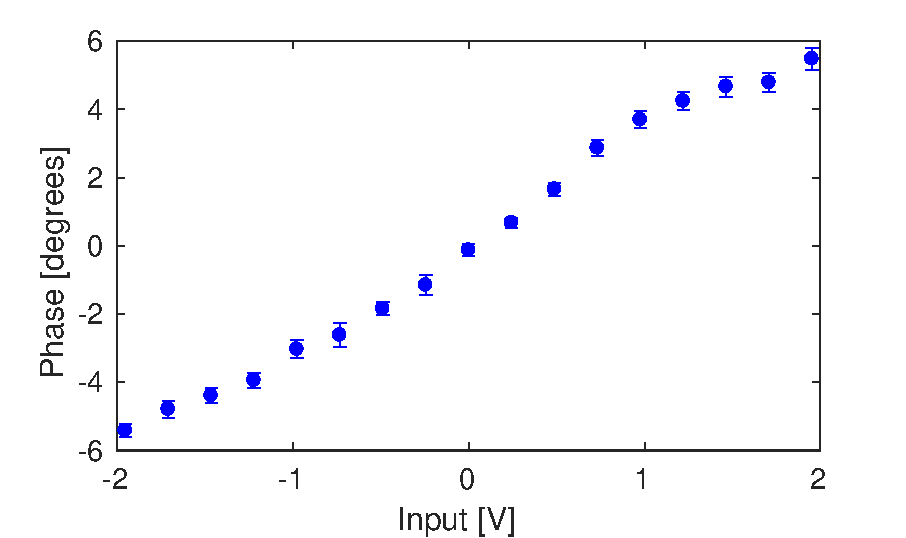
\includegraphics[width=\columnwidth]{figs/corrRange}
	\caption{\label{fig:corrRange}Downstream phase vs. the kicker amplifier 
	input voltage. Markers show the measured response, and the line a linear 
	fit to the data restricted to inputs between \(\pm1.2\)~V}
\end{figure}

The PFF system also should not degrade the transverse stability of beam after 
chicane. The purpose of the second kicker is to close the orbit bump created by 
the first kicker, so that the downstream beam orbit is independent of the 
kicker voltage. In terms of optics tranfer matrix coefficients this can be 
achieved by requiring \(R_{11}=-1\) and \(R_{12}=0\) between the 
kickers. Fig.~\ref{fig:orbClos} shows the horizontal beam orbit before, in and 
after the TL2 chicane for the maximum and minimum applied kick. The closure in 
the BPMs following the chicane is better than 0.1~mm, compared to a maximum 
offset of 1.5~mm inside the chicane.

\begin{figure}
	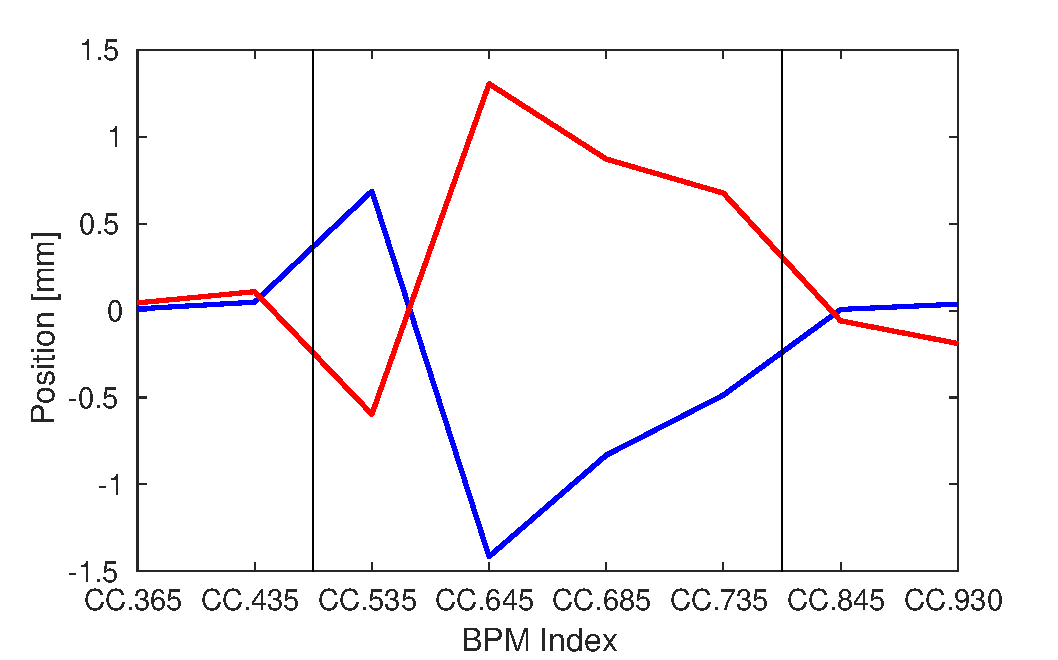
\includegraphics[width=\columnwidth]{figs/orbClos}
	\caption{\label{fig:orbClos}Horizontal orbit in and around the TL2 chicane 
	at maximum (blue) and 
	minimum (red) 
	input to the kicker amplifiers. Markers show the measured position in beam 
	position monitors, and dashed lines the predicted orbit using the 
	CTF3 MADX model and hardware parameters.}
\end{figure}

%\textcolor{red}{All this must be achieved whilst keeping dispersion low, 
%matching betas etc. 
%within constraints of pre-existing buildings. Achieved R52 0.74m with max 
%dispersion 1.16m...}

\subsection{\label{ss:r56} Phase Propagation}

The PFF system acts to subtract the measured upstream phase (\(\phi_u\)) from 
the initial downstream phase (\(\phi_d\)) with a gain factor (\(g\)):
%\begin{equation*}
\(\phi_{\mathrm{PFF}} = \phi_d - g\phi_u\)
%\end{equation*}
, where \(\phi_{\mathrm{PFF}}\) is the corrected downstream phase. The optimal 
system gain is given by:
\(g = \rho_{ud} \sigma_d/\sigma_u\)
, where \(\sigma_u\) and \(\sigma_d\) are the initial upstream and downstream 
phase jitter respectively, and \(\rho_{ud}\) is the correlation between the 
upstream and downstream phase. The theoretical limit on the corrected 
downstream phase jitter (\(\sigma_{\mathrm{PFF}}\)) with this gain is given by:
\(\sigma_{\mathrm{PFF}}=\sigma_d \sqrt{1-\rho_{ud}^2}\). 

One of the key challenges in operating the PFF prototype at CTF3 has been 
obtaining high correlation between the initial, uncorrected, upstream and 
downstream phase. A correlation of 97\% is required to reduce a typical initial 
phase jitter of \(0.8^\circ\) to the target of \(0.2^\circ\). Early 
measurements showed below 40\% correlation, and typically a factor 3 increase in the downstream phase jitter with respect to the upstream jitter.

The source of low correlation and jitter amplification was discovered to be energy dependent phase 
jitter introduced between the upstream and downstream phase monitors. This is 
described via the optics transfer matrix coefficient \(R_{56}\):
\(\phi_d = \phi_u + R_{56}(\Delta p / p)\)
, where \(\Delta p / p\) is the relative beam energy offset.

%\textcolor{red}{Correlation or jitter vs. R56 equation?...}

To achieve high upstream-downstream phase correlation the PFF system requires \(R_{56}\) to be zero between the upstream and 
downstream phase monitors.
\begin{figure}
	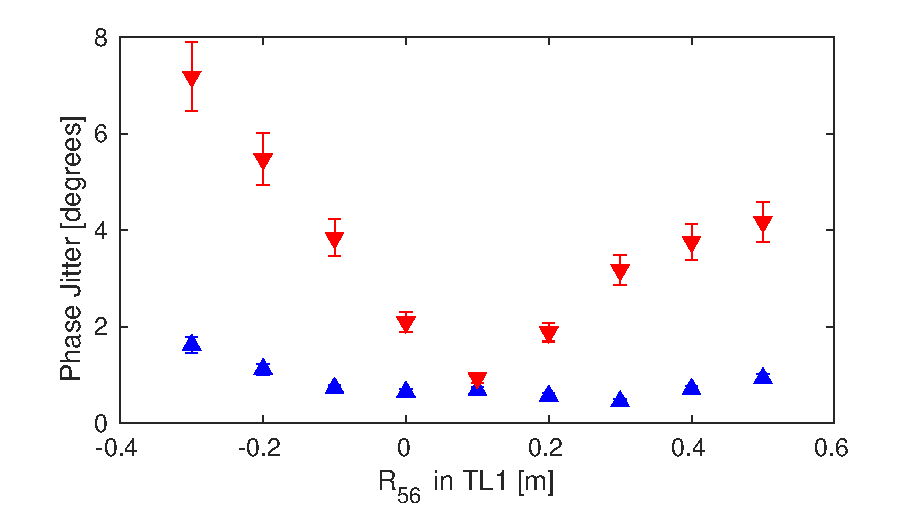
\includegraphics[width=\columnwidth]{figs/r56Scan}% Here is how to import 
	%EPS art
	\caption{\label{fig:r56Scan}Downstream (red points) and upstream (blue 
		points) phase jitter vs. the \(R_{56}\) value in the set TL1 optics. 
		}
\end{figure}

The phase propagation has therefore been optimised by creating new optics for the transfer line TL1 (see Fig.~\ref{fig:pffLayout}) with \(R_{56}\) values ranging between -30~cm and +60~cm in 0.5~cm increments. TL1 can then be used to compensate for the non-zero \(R_{56}\) values in other beam lines, with the dominant contribution being from the TL2 chicane. In other words, TL1 is tuned such that \(R_{56}(\mathrm{TL1}) = -R_{56}(\mathrm{TL2})\).

Fig.~\ref{fig:r56Scan} shows the effect of varying the \(R_{56}\) value in TL1 
on the downstream phase jitter. With an \(R_{56}\) of around 10~cm in TL1 the 
downstream phase jitter is reduced to the same level as the upstream jitter, as 
desired. The upstream-downstream phase correlation is also increased in these 
conditions, with correlations above 95\% achieved.

In this way the necessary initial conditions for the PFF correction were 
obtained at CTF3. However, the optics at CTF3 also contain a large second order 
phase-energy dependence, which leads to a degradation in upstream-downstream 
phase correlation if there are drifts in beam energy. Energy drifts resulting 
from instabilities and trips of klystrons at CTF3 have therefore made it 
difficult to maintain high phase correlations for timescales longer than 
10~minutes. 

\section{\label{s:results}Results}

\subsection{\label{ss:gScan}Gain Scan}

With the optimal gain the PFF correction acts to remove all correlation between 
the upstream and downstream phase, reducing the downstream phase jitter. If the 
gain is too small some residual correlation will remain, and if it is too large 
the correlation will flip sign. 

The optimal system gain can be derived empirically by observing the dependence 
of the downstream phase on the upstream phase with the correction on, as seen 
in Fig.~\ref{fig:gScan}. Optimal gain values for the system are typically in 
the range 1.0--1.5, being larger than unity when the downstream jitter is 
larger than upstream, as per the predicted theoretical values. 

\begin{figure}
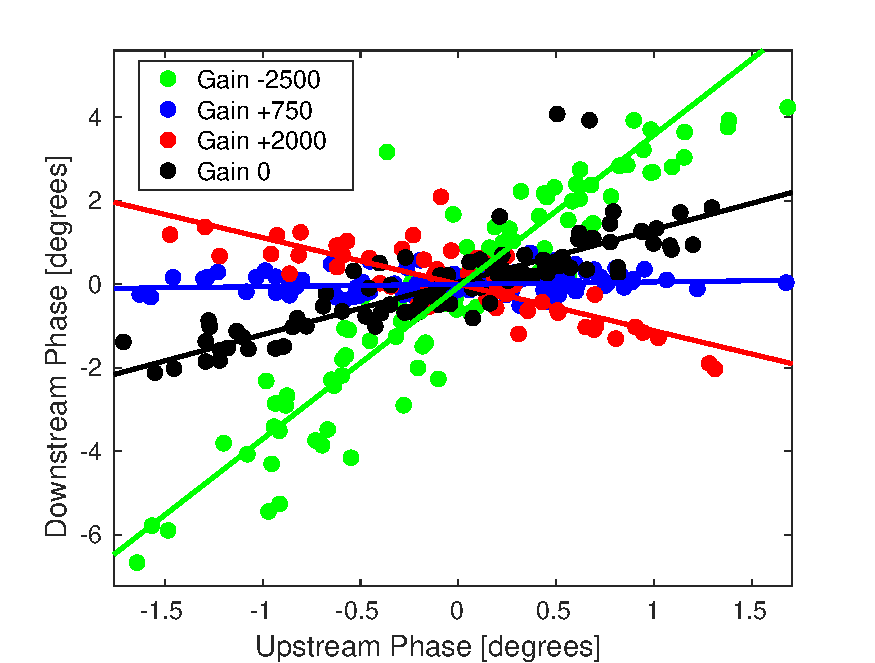
\includegraphics[width=\columnwidth]{figs/gScan}% Here is how to import EPS art
\caption{\label{fig:gScan}Downstream phase vs. the upstream phase with the PFF 
system on at four different gains: -1.6 (green), 0.0 (magenta), +1.6 (blue) and 
+3.2 (orange). Data points (markers) and linear fits to the data (lines) are 
shown.}
\end{figure}

\subsection{\label{ss:shape}Intra-Pulse Phase Variations}

The PFF correction is shaped to remove phase variations along the 
1.2~\(\mathrm{\mu s}\) CTF3 beam pulse. The predominant intra-pulse feature at 
CTF3
is a roughly parabolic ``phase sag'' of \(40^\circ\) peak-to-peak, resulting 
from the use of RF pulse compression. As this is much larger than the 
\(\pm 6^\circ\) range of the PFF system, only approximately a 400~ns portion of 
the pulse can be optimally corrected. The phase sag would not be present at 
CLIC, where in any case the drive beam pulse length is less than 400~ns.

%2015: (Peak-to-peak variation of 5.76 degrees in initial phase reduced to 
%0.65 degrees in corrected phase -- OR -- standard deviation of phases reduced 
%from 1.68 to 0.26 degrees...).

%2016: Std \(0.960\pm0.003^\circ\) reduced to \(0.285\pm0.004^\circ\) across 
%440~ns portion of pulse. Worse absolute but better removal small features 
%compared to 2015.

\begin{figure}
	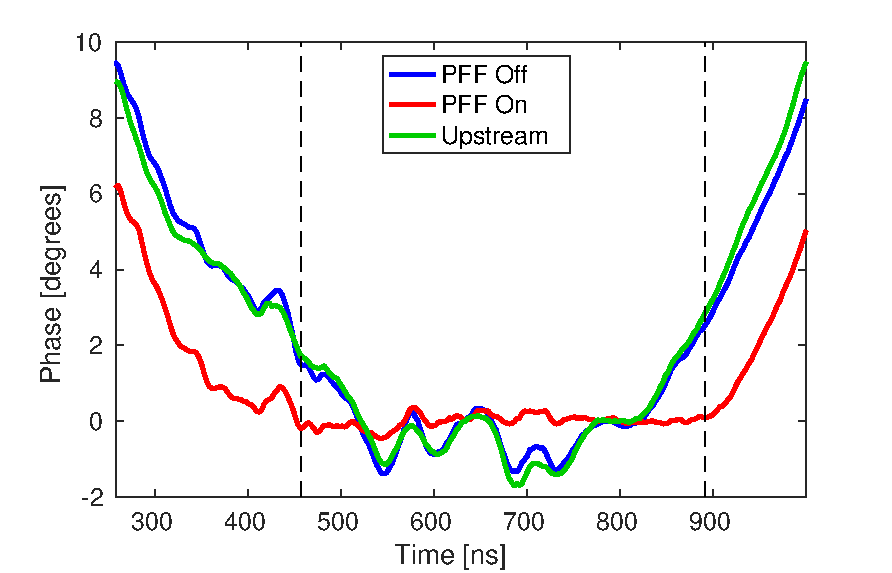
\includegraphics[width=\columnwidth]{figs/shape}% Here is how to import EPS 
	%art
	\caption{\label{fig:shape}Effect of the PFF system on intra-pulse phase 
		variations. The pulse shape upstream (green), and downstream with the 
		PFF 
		system off (blue) and on (red) is shown.}
\end{figure}

\begin{figure}
	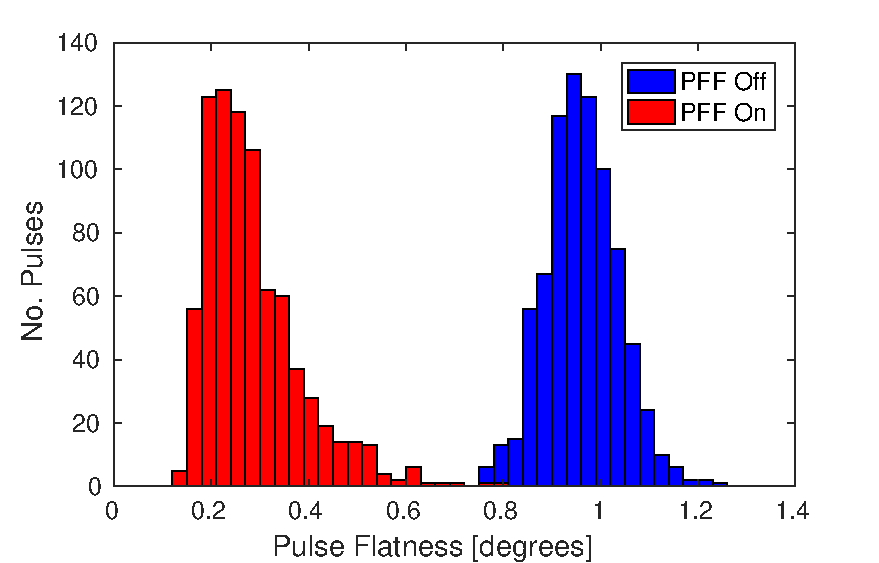
\includegraphics[width=\columnwidth]{figs/flatness}% Here is how to import 
	%EPS art
	\caption{\label{fig:flatness}Distribution of downstream rms phase values, 
		here 
		referred to as the 
		``pulse flatness'', for each beam pulse with the PFF system off (blue) 
		and 
		on (red).}
\end{figure}

Fig.~\ref{fig:shape} shows the effect of the PFF system on the intra-pulse 
phase variations. The convention at CTF3 is to operate the PFF system in 
interleaved mode, with 
the correction applied to alternating pulses only. This allows a measurement of 
the initial (`PFF Off') and corrected (`PFF On') downstream phase to be 
performed concurrently. The upstream (PFF input) phase is also shown for 
comparison. Vertical dashed lines mark a 440~ns portion of the pulse where the 
correction is optimal, and this range is used to calculate statistics on the 
effect of the system. 

In this range the PFF system flattens the phase, 
and almost all variations are removed. Residual offsets in the phase are still 
present where there are small uncorrelated differences between the shape of the 
initial upstream and downstream phase. Fig.~\ref{fig:flatness} shows the rms 
phase variation within the 440~ns range 
for each beam pulse in the dataset, with the PFF system on and off. The PFF off 
pulses have an rms of \(0.960\pm0.003^\circ\) on average, and this is reduced 
to \(0.285\pm0.004^\circ\) by the PFF system.

The PFF system at CTF3 has been verified to reduce the amplitude of 
phase errors up to a frequency of 25~MHz, exceeding the CLIC requirements.


%Limited by variations in phase propagation along the pulse (energy differences 
%etc.).

\subsection{\label{ss:meanJit}Pulse-to-pulse Jitter}

As well as removing intra-pulse phase variations the PFF system simultaneously 
corrects offsets in the overall mean phase, i.e. any pulse-to-pulse jitter. The 
mean phase of each beam pulse is calculated across the 440~ns range in the 
central portion of the pulse, as shown before in Fig.~\ref{fig:shape}.

\begin{figure}
	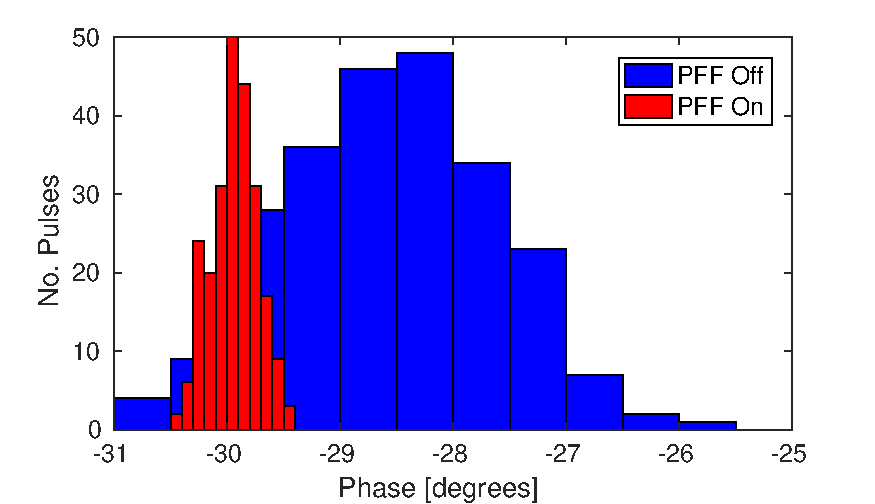
\includegraphics[width=\columnwidth]{figs/meanJit}% Here is how to import 
	%EPS 
	%art
	\caption{\label{fig:meanJit}Distribution of the mean downstream phase with 
		the 
		PFF system off (blue) and on (red).}
\end{figure}

Fig.~\ref{fig:meanJit} shows the effect of the PFF system on the pulse-to-pulse 
stability across a dataset around ten minutes in length. An 
initial mean downstream phase jitter of \(0.92\pm0.04^\circ\) is reduced to \(0.20\pm0.01^\circ\) by the PFF 
correction. All correlation between the upstream and downstream jitter is removed, from 
\(96\pm2\%\) to \(0\pm7\%\). The achieved stability is consistent with the theoretical prediction (considering the initial correlation and jitter) of \(0.26\pm0.06^\circ\) within error bars.
%\textcolor{red}{NB: upstream PFF off is \(0.76\pm0.03^\circ\), but 
%\(0.68\pm0.03^\circ\) for 
%PFF on. Helps to explain why achieved is better than predicted.}

This represents the longest time period during which the target CLIC phase 
stability has been achieved with the prototype. \(0.30^\circ\) phase jitter has 
been achieved in 20 minute datasets. The limiting factor for achieving this 
performance on longer timescales is the incoming beam conditions; in particular 
klystron instabilities at CTF3 lead to degraded upstream-downstream phase 
correlation and phase drifts outside the PFF correction range, as previously 
mentioned.

The PFF system has also been operated 
whilst intentionally varying the incoming mean phase, as shown in 
Fig.~\ref{fig:wiggle}. The PFF system removes the additional phase variations 
and achieves more than a factor 5 reduction in downstream phase jitter, from 
\(1.71\pm0.07^\circ\) to \(0.32\pm0.01^\circ\) in this case.

\begin{figure}
	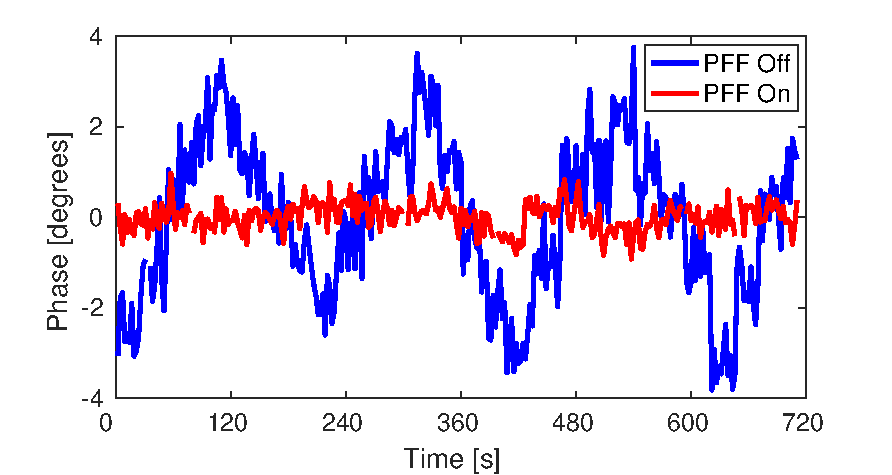
\includegraphics[width=\columnwidth]{figs/wiggle}
	\caption{\label{fig:wiggle}Mean downstream phase with the PFF system off 
		(blue) and on (red) vs. time, with additional phase variations added to 
		the 
		incoming phase.}
\end{figure}

%\subsection{\label{ss:pbpJit}Point-by-point Jitter}
%
%\textcolor{red}{I would remove this. Don't think it adds any 
%information beyond mean jitter and correction of shape.}
%
%\begin{figure}
%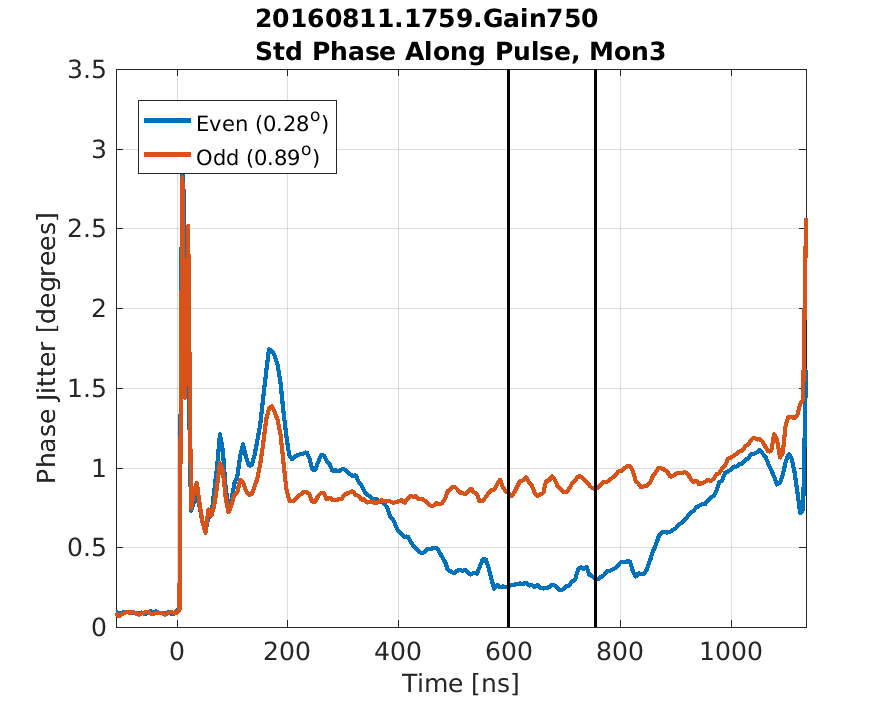
\includegraphics[width=\columnwidth]{figs/BestFF_pbp}% Here is how to import 
%%%%EPS art
%\caption{\label{fig:BestFF_pbp}Point-by-point jitter.}
%\end{figure}
%
%Point-by-point jitter of x~degrees achieved across a x~ns portion of the 
%pulse, agrees with simulated value...

\section{\label{s:conc}Conclusions}

CLIC requires a PFF system to reduce the drive beam phase jitter by an order of 
magnitude, from \(2.0^\circ\) to \(0.2^\circ\)~at~12~GHz, or better than 50~fs 
stability. A prototype of the system has been 
in operation at the CLIC test facility CTF3, and corrects the beam phase by 
varying the path length through a chicane using two electromagnetic kickers. 

As 
well as the kickers, the system uses newly designed phase monitors with 
\(0.12^\circ\) resolution, high bandwidth 20~kW amplifiers and a low latency 
digitiser/feedforward controller. The system latency, including hardware and 
signal transit times, is less than the 380~ns beam time of flight between the 
input phase monitor and the correction chicane. Therefore, the feedforward 
correction can 
be directly applied to the same bunch initially measured at the monitor.

New optics for the correction chicane and other beam lines at CTF3 have been 
developed to yield the desired phase shifting behaviour and ensure high 
correlation between the initial upstream and downstream phase.

The prototype system has demonstrated \(0.20\pm0.01^\circ\) pulse-to-pulse 
phase jitter on a time scale of ten minutes. It has also been shown to be able 
to flatten intra-pulse phase variations up to a frequency of 25~MHz. On longer 
timescales the performance of the system is limited by changes to the incoming 
beam conditions, in particular beam energy, which would be better controlled in 
any future application at CLIC.

%Drifts, in particular in beam energy, degrade the correlation between the 
%upstream and downstream phase and prevent this level of stability from being 
%demonstrated on longer time scales at CTF3. A key consideration for any future 
%system should be to design beam lines and optics with zero phase-energy 
%dependence, including non-linear dependencies, to solve this issue.

%\textcolor{red}{Try to apply to XFELs/something else.}

\section{\label{s:ack}Acknowledgements}
\begin{acknowledgments}
	We wish to acknowledge everyone involved in the operation of CTF3 for their 
	help and support in realising the PFF system.
\end{acknowledgments}

\bibliography{pff_short}% Produces the bibliography via BibTeX.

\end{document}
